\chapter{绪论}

\section{研究背景}
% 机器翻译的大背景
眼睛帮助人类认识世界,语言则是人类互相交流的手段,人类在认识世界和传递信息的过程中离不开语言和视觉的相互配合。随着全球化的发展,不同国家不地区的人们也急迫着去了解更多的新鲜事物,体察不同的风俗人情,感受世界的动荡与变化。然而在这个过程中,语言障碍严重地影响了人们的文化交流。因此,人们对机器翻译(machine translation,MT)技术的需求变得更为迫切。

%机器翻译的历史:由传统->神经网络
机器翻译是一种利用计算机技术将一种自然语言(通常称为源语言)自动翻译成另一种自然语言(通常称为目标语言)的方法\cite{zong2013}。虽然语言之间的相互翻译是一种非常复杂的问题,但早在1949年,美国数学家沃伦·韦弗(Warren Weaver)就在其发表的著作《翻译备忘录》中就提出了机器翻译的原始构想。伴随着计算机技术的发展与相关学科的不断进步,机器翻译的相关研究也在逐渐地深入。机器翻译经历了基于规则的方法、基于实例的方法以及统计机器翻译等多次技术上的革新。随着近年来计算机算力的不断的突破,深度学习方法逐步走入研究者们的视野,神经机器翻译(neural machine translation,NMT)\cite{kalchbrenner-blunsom-2013-recurrent,1_DBLP:journals/corr/SutskeverVL14,3_DBLP:journals/corr/BahdanauCB14}方法也展现出其独有的特点。NMT方法不仅是目前学术研究所采用的主流翻译框架,同时也在商业应用上展现了其无限的潜能。目前,谷歌、微软、百度等国内外公司均在其在线翻译系统中应用了NMT模型框架,为世界不同地区的人们提供优质、免费的翻译服务。

%神经网络方法是自然语言处理与计算机视觉的交汇点->多模态机器翻译
神经网络不仅是当前机器翻译的基础方法,更是在整个自然语言处理,以及计算机视觉和语音识别等领域均得到了突破性的应用。虽然不同的研究领域采用了不同的网络框架,但是神经网络方法具有统一的分布式向量表示、反向传播、深度网络结构等方法范式。这使得不同领域的方法以及来自不同模态的信息在此形成了交汇点。而机器翻译也可以脱离常规的以单个句子为翻译单位的任务范式。多模态机器翻译(multi-modal machine translation,MMT)就是一种通过融合不同模态信息(如视觉信息、语音信息、篇章信息等)帮助自然语言的语音或文本进行翻译的一类方法。本文将聚焦融合图片信息的神经机器翻译(image-incorporated neural machine translation,ImgNMT)方法展开研究工作。

%举例:多义词,歧义词,语义不完整,
\begin{figure}[!htbp]
    \centering
    \begin{subfigure}[b]{1\linewidth}
      \centering
      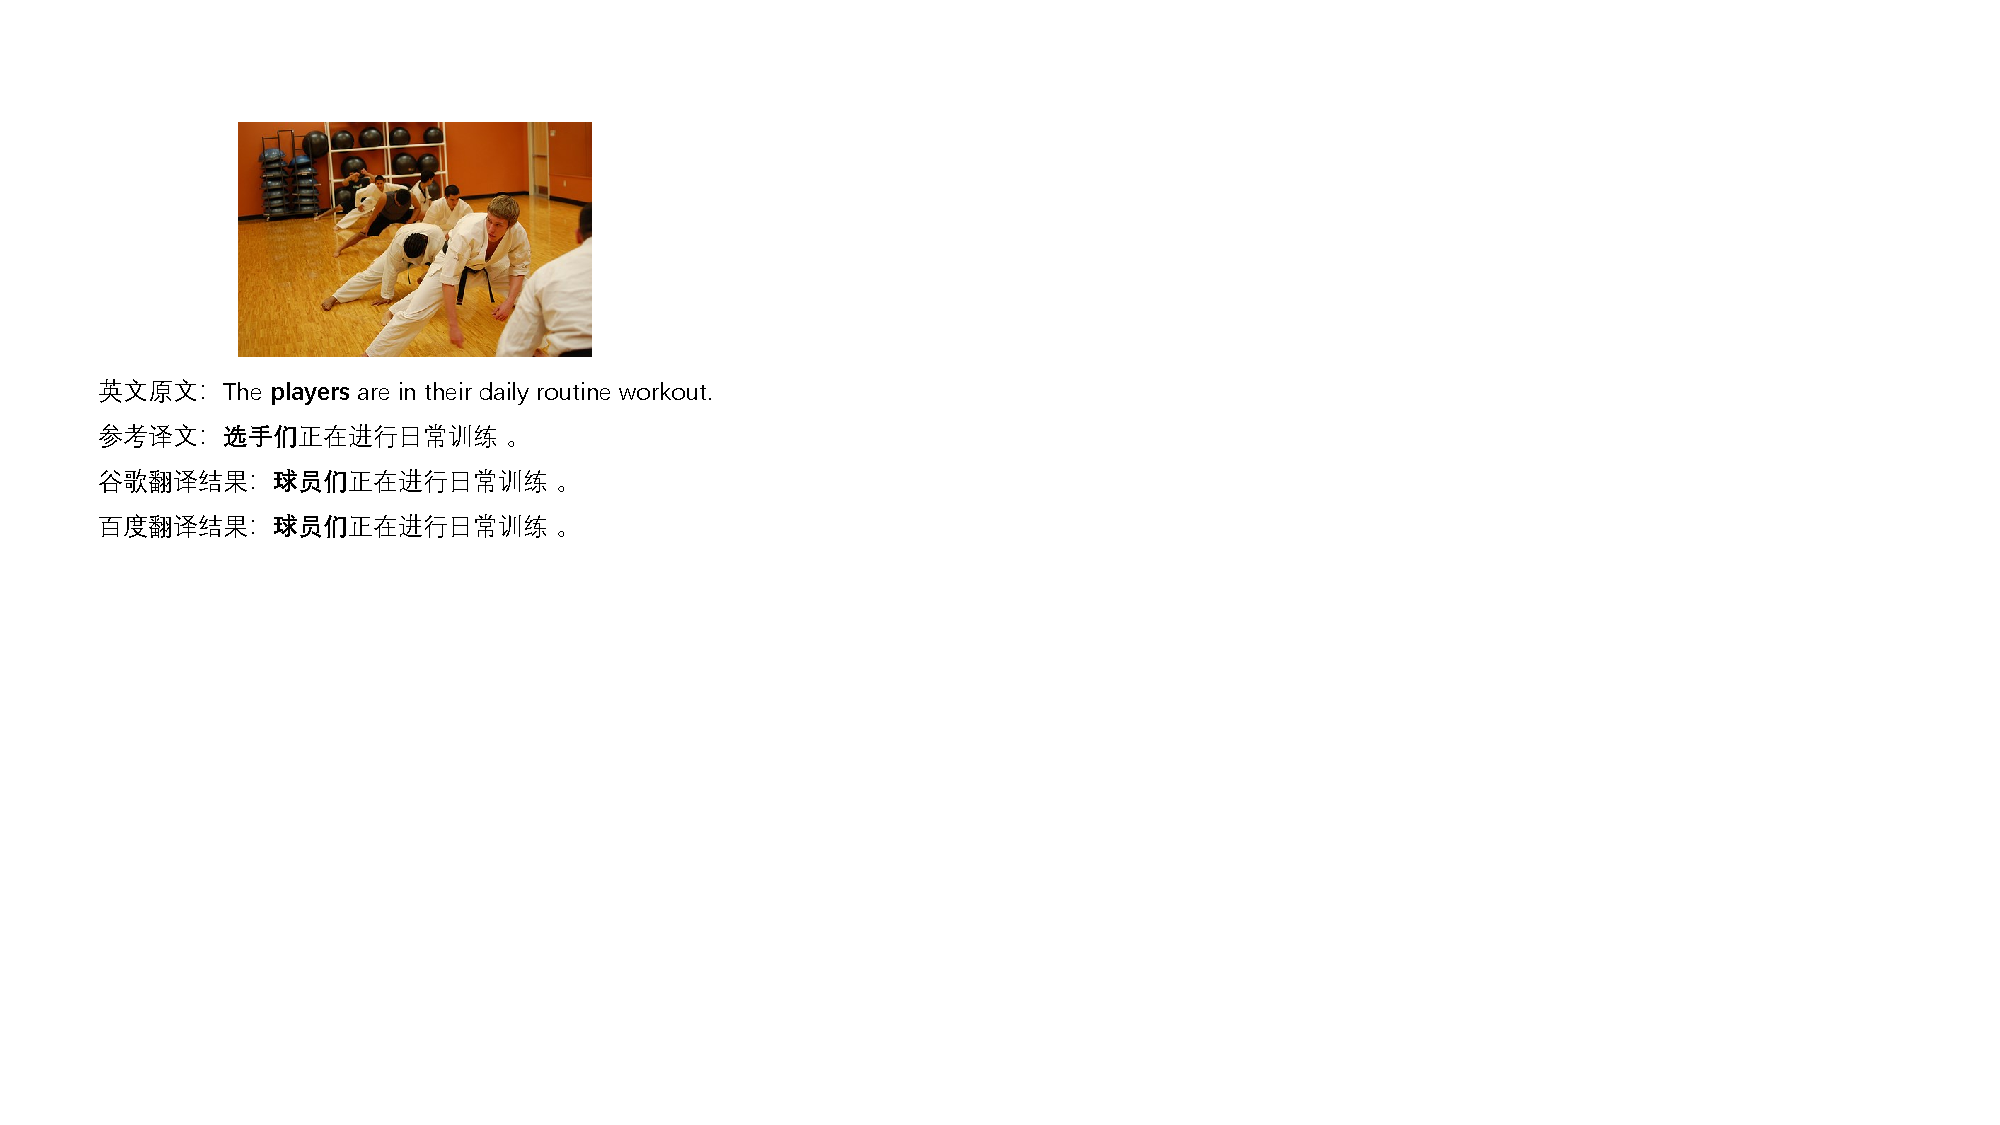
\includegraphics{Img/fig_1_case_players.pdf}
      \caption{错翻单词“players”}
      \label{fig:1_players}
    \end{subfigure}%
    \\
    \begin{subfigure}[b]{\linewidth}
      \centering
      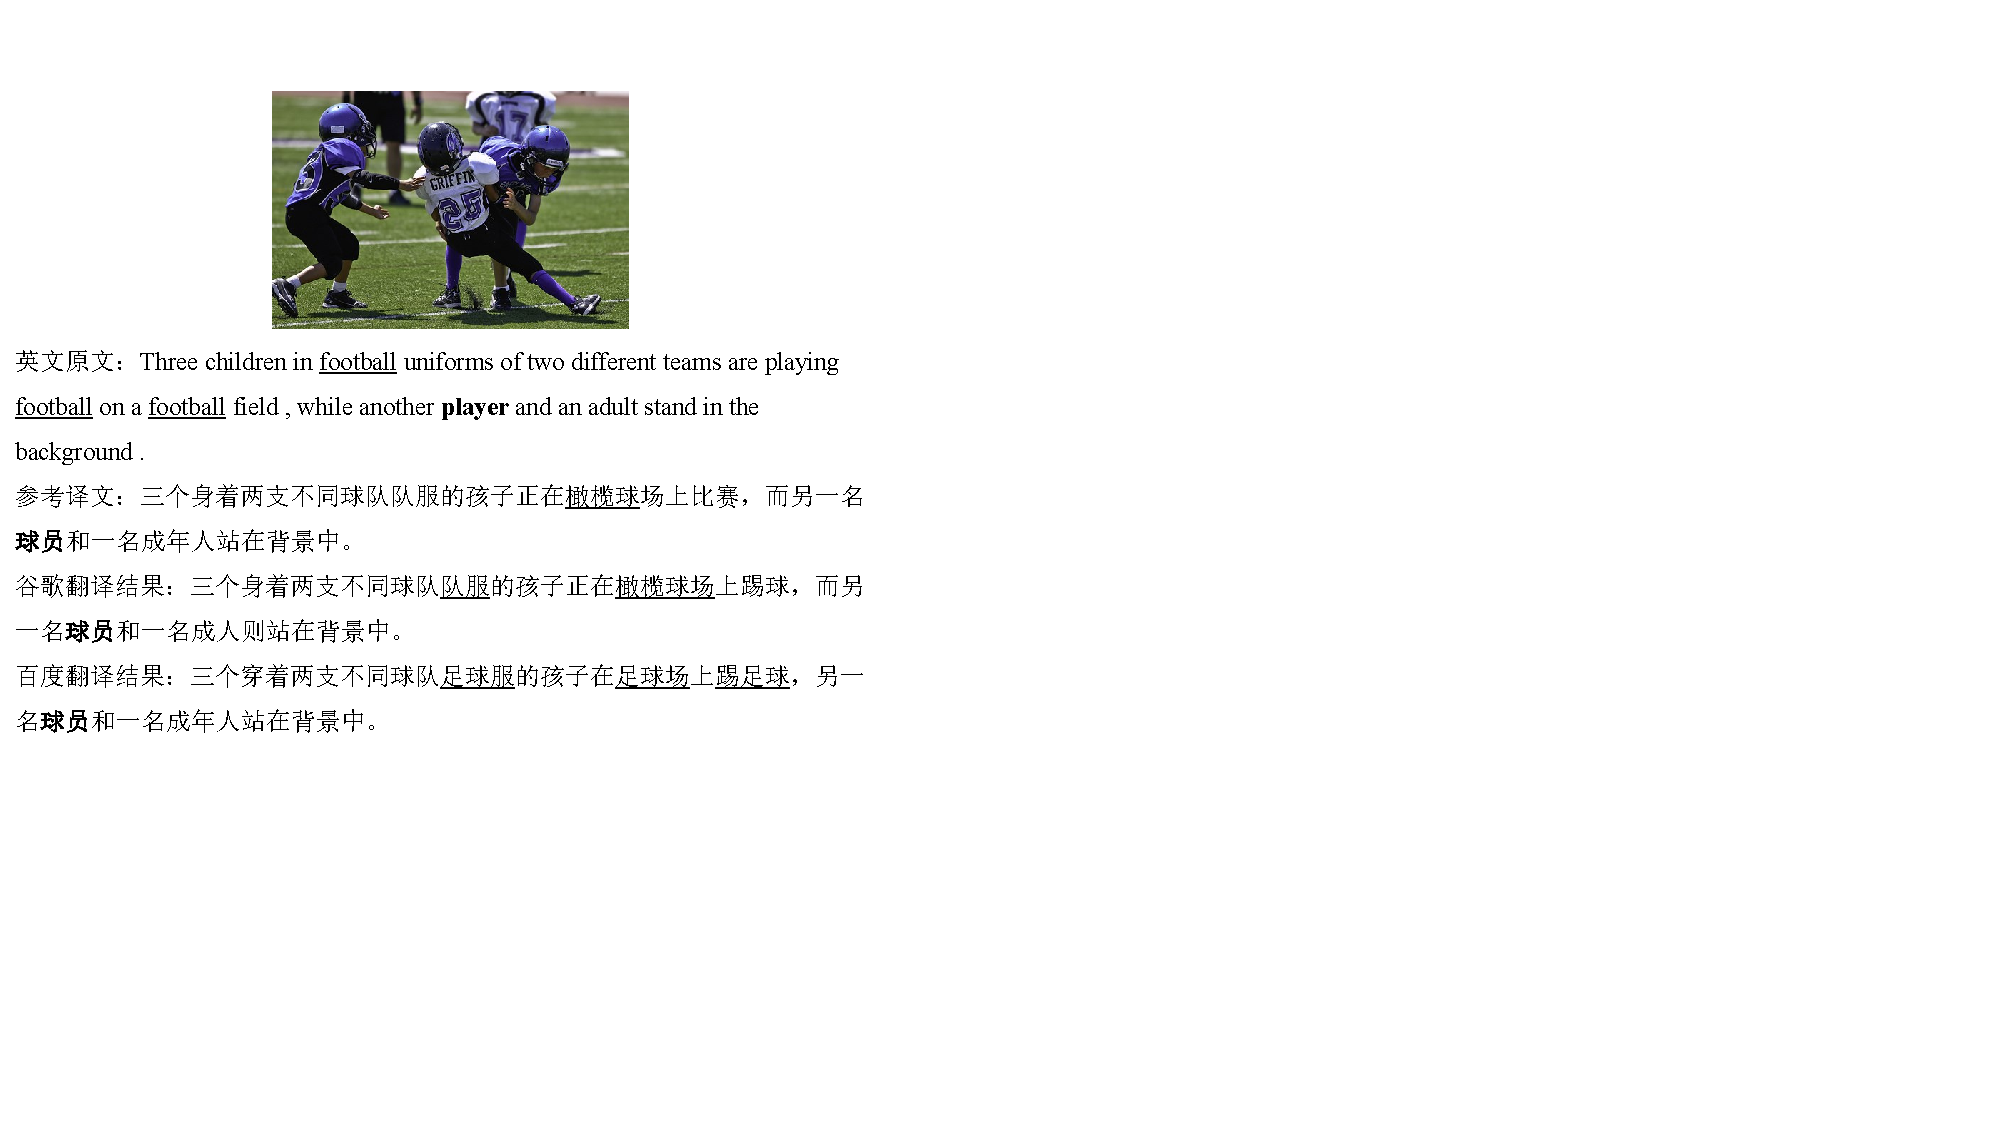
\includegraphics{Img/fig_1_case_football.pdf}
      \caption{错翻单词“football”}
      \label{fig:1_football}
    \end{subfigure}
    \bicaption{翻译错误案例}{Cases of incorrect translation}
    \label{fig:1_translation_cases}
\end{figure}
图\ref{fig:1_translation_cases}给出了谷歌和百度的机器翻译系统对两句英文图片描述的翻译结果。
在图\ref{fig:1_players}中展示了一个简单却缺少上下文信息的翻译例子,加粗项“players”在实际应用中随着背景信息的变化可以有多种不同的释义,在图例中应指的是“空手道选手们”。然而,在不考虑图片所提供信息的情况下,两个纯文本机器翻译系统均将其翻译为更常见的释义“球员们”。仅从文本的角度考虑,该翻译结果并不差,但因为文本所提供的信息是不完整的导致其翻译结果与真实释义存在一定的差距。
图\ref{fig:1_football}的例子中同时包含了“football”(下划线项)和“player”(加粗项)两个容易翻译错误的地方。从谷歌和百度翻译系统的结果中可以看到,在不提供图片信息的情况下,谷歌翻译系统将“football”翻译为“橄榄球”,而百度翻译系统将其翻译为“足球”。在未提供图片信息的情况下,不同的翻译系统表现出了不同的倾向性,仅从文本信息的角度两者都是正确的翻译。在图\ref{fig:1_football}的例子中“player”翻译到了正确的“球员”释义。其原因可以归结为两点,一是如同图\ref{fig:1_players}的例子一样,翻译系统选择了更为常用的“球员”释义;二是翻译系统捕捉到了整段原文中提供的有关于“球”的上下文信息,从而得到了正确的翻译。


上述例子表明,当句子中存在多义词、歧义词、语义不完整等问题时,图片中所包含的视觉信息能够作为翻译过程中所需要的上下文信息,而常规的神经机器翻译系统不具备建模和利用来自其它模态的信息的能力。在真实的应用场景中,翻译系统要处理的可能是商品介绍、聊天记录、网络简讯等有匹配图文的句子。因此,探索融合图片信息的神经机器翻译方法具有重要的理论研究和实际应用价值。图片中包含着更丰富、更完整以及更准确的信息能够为句子的翻译提供更适合的上下文语境,帮助模型得到优化的编码表示,或是为模型解码提供视觉信息作为参考。

相比于统计机器翻译,在神经机器翻译中融合来自图片中的信息是更方便且更自然的,这也推动了ImgNMT的研究热潮,相关研究大量涌现。目前的ImgNMT方法主要关注针对图片描述的翻译中,如何利用图片信息改进翻译质量。图片描述的翻译任务中,句子与图片具备语义上的一致性,图片与句子之间语义融合的研究可以从更多的角度展开,其相关研究成果与结论也可以更方便的应用到其它领域。相关的模型方法主要关注图片信息在神经机器翻译模型中的利用,提出了各具特点的网络结构以及采用各种图片输入方式来建模视觉上下文信息,从而方便图片信息在神经机器翻译模型中的利用。然而,神经网络方法为跨模态信息融合带来便利的同时,也极大地削弱了各种模型方法的可解释性。存在大量的方法对翻译质量的提升有限,但却因为图片信息作用方式不明确的原因,难以进行针对性的改进。另外,NMT所采用的平行翻译数据一般具有良好的语义对齐特性。相比之下,句子与图片之间的语义对齐关系则更为复杂。这使得一般的ImgNMT模型在训练阶段很容易收敛为一个忽略了图片信息的纯文本翻译模型,导致模型在应用测试阶段也仅是将输入的图片输入作为噪声。
因此,本文主要从模型层面出发,针对目前融合图片信息的神经机器翻译方法利用图片信息方式的缺陷,探索更有效的跨模态信息融合方法,从而提升神经机器翻译的译文质量。


\section{研究内容}

本文的研究旨在改善目前融合图片信息的神经机器翻译方法中图片信息的作用方式,提升图片与文本在语义融合过程中的作用程度,从而达到提升译文质量的目的。本文的研究内容主要包括:如何将图片信息明确地作用在句子中的对应目标;如何进一步改进明确的视觉信息作用方式,将其与常规的跨模态信息融合方法相结合;如何提升常规跨模态信息融合方法中图片信息的作用程度,利用更多的视觉信息改善翻译质量。

具体地,本文的主要工作可以划分为以下三个部分:

{\sffamily 1. 基于跨模态文本重构的神经机器翻译方法}

% 面对什么问题
主流的融合图片信息的神经机器翻译方法将图片输入到经过特殊设计的翻译模型中,利用神经网络方法具有直接从数据中学习数据特征的优点,实现将图片信息融合到句子的翻译中。但这种方法并不能保证图片在模型中的有效性,部分方法甚至不会为模型带来性能的提升。并且,图片信息的作用方式不明确,导致难以对方法实施针对性的改进。
%将图片输入到神经机器翻译模型中具有直接从数据中学习并融合跨模态信息的优点,但也难以明确图片信息的具体作用,因此这类方法可称为隐式跨模态信息融合法。
% 如何解决
为了探究显式跨模态信息融合法是否可行,本文提出一种基于跨模态文本重构的神经机器翻译方法。
% 具体怎么做
该方法将一个文本重构任务与翻译任务相结合,将文本重构任务作为辅助任务来提升翻译性能。在训练过程中,该方法首先使用视觉目标来替换源语言句子中与图片相关的部分,然后使用一个端到端生成式模型来恢复原始句子或生成目标语言句子。然后采用了参数共享机制,使得生成式模型在两个任务之间共享编码器或解码器部分,从而实现了对翻译模型的有效增强。
%该方法将一个文本重构任务与翻译任务相结合。文本重构模型在训练中将源语言句子中的名词或短语的位置明确地替换为图片中对应的视觉目标,并将该序列输入并重构到完整的源语言句子或目标语言的句子。由于文本重构模型也是端到端的文本生成式模型,因此可以通过参数共享的方式将重构模型编码器或解码器的参数与翻译模型共享,最终达到增强翻译模型的目的。
% 实验效果
实验表明,本文所提出的文本重构方法在测试阶段不需要输入图片的情况下有效地提升了模型的性能。并且该方法能够明确视觉信息为实体词的翻译带来了提升。

{\sffamily 2. 基于双向跨模态实体重构的神经机器翻译方法}

%面对问题
显式跨模态信息融合法能够将视觉信息明确地作用在词级或短语级的跨模态信息融合中。隐式跨模态信息融合方法主要作用在句子级别的语义融合。仅采用文本重构方法一方面只应用了图像到文本单方向重构,另一方面视觉信息仅作用到了实体词上,可以进一步增加句子级别的语义融合。
%如何解决
为了将显示跨模态信息融合方法与隐式方法相结合,本文提出一种基于双向跨模态实体重构的神经机器翻译方法,并将其与文本非实体重构方法相结合。
%具体做法
为了避免在重构过程中产生冗余信息,本文提出了一种新颖的跨模态信息融合方法,它放弃了对整个源语言句子的重构,而只针对实体和非实体进行不同类型的重构。实体重构代表着从文本实体中重构视觉实体和从视觉实体中重构文本实体的双向重构。文本非实体重构代表从文本上下文和视觉实体所组成的跨模态上下文中重构文本非实体。将双向重构与文本非实体重构三个任务和翻译任务融合为一个多任务学习框架,并提升翻译模型的性能。
%文本重构方法在重构的过程中生成了源语言端已经提供的信息。因此本文所提方法抛弃了文本级别的重构,在文本实体和视觉实体之间做双向的实体级重构。并增加了非实体的重构,使图片信息与文本上下文做进一步的信息融合。然后,将以上三种重构任务与翻译任务通过多任务学习的方式结合。
%实验结果
实验表明,该方法进一步地提升了机器翻译的质量。实验分析表明,双向实体重构与非实体重构的多任务组合方式使模型受益最大,说明显式方法与隐式方法的结合是有效的。

{\sffamily 3. 基于图文对比对抗训练的神经机器翻译方法}

%面对的问题
前两部分工作采用了图片增强式的神经机器翻译方法,利用多任务参数共享机制,将显示和隐式跨模态信息融合方法学习到的图片信息作用到翻译模型的参数优化中。但此类方法存在图片信息利用不充分的问题。将图片输入到翻译模型中的图片信息辅助式的神经机器翻译方法能够解决这个问题,但这类方法普遍存在模型对视觉信息不敏感的问题。
%如何解决
针对此问题,本文提出一种基于图文对比对抗训练的神经机器翻译方法。
%具体做法
为了增强模型对图片信息的利用,需要在模型训练过程增加一个图文语义匹配的功能。为此采用了对比学习方法,拉近翻译模型的图文对与译文在文本表示空间中的语义关系。然后再向负样本集中加入对抗样本。该对抗样本是将原图文对中的图片用随机的错误图片替换,使原文同时出现在正负样本集中。但因为输入的图片不一致,模型在对比学习的训练过程中需要将图片信息融合到文本表示中才能判断样本的正负性,并以此达到融合图片信息的目的。
%为了拉近双语的语义关系,在编码端增加了图文与目标语言句子之间对比学习。并在负样本集中引入了包含源语言句子+错误图片对抗样本。为了将正负样本区分开,模型需要判断图片信息是否与源语言句子的语义一致。该方法会将图片信息融合到文本的表示中,从而提升视觉信息在模型中的作用程度。
%实验结果
实验结果表明,该方法提升模型翻译性能的同时还提升了模型对视觉信息的敏感度,输入正确图片的翻译结果明显优于输入错误或不输入图片的情况。


\section{论文的组织结构}

围绕上述研究内容,本文共分为六章,具体的组织方式如下:

第1章为绪论部分。本章首先机器翻译以及融合图片信息的神经机器翻译的研究背景和意义进行介绍,并指出神经机器翻译方法在融合图片信息的过程中存在哪些问题,随后介绍了本文针对目前存在问题所做的研究内容,最后在本节介绍了论文的组织结构。

第2章为融合图片信息的神经机器翻译方法国内外研究现状。本章首先详细介绍了神经机器翻译模型的发展历程和基础的模型框架。然后介绍了在将图片信息传递给神经机器翻译模型前,有哪些计算机视觉基础模型可以为跨模态信息的融合提供便利。紧接着,对融合图片信息的神经机器翻译方法进行了分类介绍,包括图片信息辅助式方法、图片信息增强式方法、基于图片搜索的方法以及无监督方法。最后,分析了现有方法所面临的问题与挑战,进而引出本文所要开展的工作。

第3章介绍了基于跨模态文本重构的神经机器翻译方法。为了将图片信息明确地作用到文本中的对应目标上,本章首先介绍了图片中的视觉目标与文本中的词或短语的对齐方法,设计了图片目标在文本编码过程中的明确作用方式。然后设计了两种文本重构方案和三种参数共享方案将重构任务融合到文本翻译任务中。最后介绍了所提方法在英德翻译数据上的实验结果。

第4章介绍了基于双向跨模态实体重构的神经机器翻译方法。为了进一步挖掘采用明确方式融合图片信息方法的潜能,本章首先介绍了文本实体到图片实体和图片实体到文本实体两个方向的实体级重构方案。为了充分利用图片中的视觉信息,将视觉信息与文本上下文融合,本章还介绍了非实体的重构方案。然后将以上三种重构方法以多任务学习的方式与翻译任务相结合。最后介绍了此多任务方法在三个翻译对上的有效性。

第5章介绍了基于图文对比对抗训练的神经机器翻译方法。为了在图片与文本信息融合过程中,使模型对图片中所包含的信息更敏感,本章首先介绍了一种在对比学习中加入对抗样本作为负样本的方法。然后在多个语言对上测试了所提方法提升翻译准确率的能力。最后分析了,对比对抗训练方法能否提升图片在神经机器翻译中的作用。

第6章对本文的研究工作进行总结,分析现有研究工作的不足,并对未来的研究工作进行展望。